A partir da revisão 1.1 são adicionados mecanismos opcionais para garantir a segurança dos dados trafegados no barramento, incluindo privacidade de objetos e também verificação de identidade do mestre.

\section{Autenticação de mestre}

Este recurso é utilizado para garantir a autenticidade dos comandos enviados aos dispositivos no barramento. Comandos de RESET e escrita em objetos são assinados digitalmente, caso o dispositivo suporte a autenticação.

Isto garante que mesmo no caso de um dispositivo malicioso ser conectado ao barramento, os dispositivos seguros não possam ser instruídos a realizar operações que possam ser danosas ao sistema.

\subsection{O mecanismo de autenticação}

Se o dispositivo suporta autenticação, o mestre deve inserir um bloco de dados após os comandos que necessitam da verificação de identidade.

O dispositivo que suporta autenticação é chamado de \textit{seguro} e o que não suporta de \textit{inseguro}.

Os dispositivos seguros só podem executar os comandos que necessitam de autenticação uma vez que seja verificada a autenticidade da mensagem através do bloco de assinatura.

Um dispositivo seguro descarta os comandos recebidos se eles não possuem o bloco de autenticação ou se a verificação de autenticidade falhou.

Da mesma maneira, os dispositivos inseguros devem ser capazes de receber comandos contendo blocos de autenticação e realizar as tarefas indicadas, ignorando o bloco de autenticação.

\subsection{O método de autenticação}

Para a autenticação são utilizados conceitos similares ao sistema criptográfico de chave pública RSA.

No caso do barramento HBUS, é escolhido um sistema com uma menor complexidade matemática, o sistema criptográfico de Rabin-Williams. Este sistema é muito similar ao sistema RSA, porém pouco conhecido. Ele é equivalente a um sistema RSA com expoente público 2.

As chaves utilizadas são de 1536 bits.

\subsubsection{O sistema criptográfico Rabin-Williams}

O sistema criptográfico de Rabin utiliza o seguinte esquema para suas chaves:

\begin{enumerate}

\item São escolhidos dois números primos p e q, obedecendo: $p \equiv 3 \mod{8}$ e $q \equiv 7 \mod{8}$.

\item $\left({}p,q\right)$ é a chave privada.

\item Calcula-se $n=p\cdot{}q$. $n$ é a chave pública.

\end{enumerate}

\subsubsection{O processo de assinatura}

O mestre realiza este processo todas as vezes que enviar uma mensagem com autenticação.

\begin{enumerate}

\item O mestre calcula $h = H\left({}m|r\right){}$, onde $m$ é a mensagem, $r$ é um número aleatório e $H\left({}\cdot{}\right){}$ é uma função de \textit{hash} pública.

\item Computa-se $U = h^{(q+1)/8} \mod{q}$.
\item Se $U^4 - h \mod{q} = 0$, $e = 1$, c.c. $e = -1$.
\item É calculado $V = \left({}eh\right){}^{(p-3)/8} \mod{p}$.
\item Se $\left({}V^4\left({}eh\right){}^2 - eh\right){} \mod{p} = 0, f = 1$, c.c. $f = 2$
\item É pré-calculado $2^{(3q-5)/8} \mod{q}$. $W = f^{(3q-5)/8}U \mod{q}$.
\item É pré-calculado $2^{(9p-11)/8} \mod{p}.$ $X = f^{(9p-11)/8}V^3eh \mod{p}$.
\item É pré-calculado $q^{p-2} \mod{p}$. Calcula-se $Y = W + q\left({}q^{p-2}\left({}X - W\right){} \mod{p}\right)$.
\item Computa-se $s = Y^2 \mod{pq}$. A assinatura da mensagem é o par $\left({}e,f,r,s\right)$, que é enviado junto a mensagem.

\end{enumerate}

\subsubsection{O processo de verificação}

Esse processo é realizado pelo dispositivo toda vez que recebe uma mensagem com assinatura.

\begin{enumerate}

\item O dispositivo recebe a mensagem juntamente com a assinatura.

\item O dispositivo calcula $efs^2 \mod{pq}$ e $H\left({}m|r\right)$ e verifica se são iguais. Sendo iguais, a assinatura é comprovada

\end{enumerate}

\subsubsection{A função de hash}

A função de hash utilizada é a bem conhecida função SHA-1. A saída da função SHA-1 tem 160 bits de comprimento.

\subsection{O custo da autenticação}

O custo da autenticação é principalmente refletido na quantidade de memória ocupada no dispositivo, tanto de programa quando RAM. Além disto, há o tempo necessário para realizar as verificações, que são baseadas em operações matemáticas um tanto pesadas para dispositivos de 8bits como é o caso dos microcontroladores utilizados no desenvolvimento da pilha HBUS.

Utilizando o processo de autenticação, o overhead de autenticação na mensagem é maior do que a própria mensagem, porém isto é uma questão de segurança e não se pode fazer nada sem comprometer a segurança do sistema.

O bloco de assinatura tem 193 bytes, onde 1 byte é dedicado ao armazenamento das variáveis e,f e r e os 192 bytes restantes são o produto do processo de assinatura realizado pelo mestre (192 bytes = 1536 bits --- tamanho das chaves). 

\section{Autenticação de dispositivo}

O caminho inverso é também possível e desejável em casos que o nível de segurança deve ser maior. No entanto, o sistema de autenticação é assimétrico e a assinatura é muito mais custosa que a verificação. Devido a este fator limitante, a autenticação de dispositivos é possível apenas para dispositivos que utilizem-se de outras soluções mais poderosas que microcontroladores de 8 bits.

Esta é uma funcionalidade futura da especificação HBUS.

\subsection{Requisitos e guia de implementação}

Nesta modalidade de autenticação, cada dispositivo que possuir a capacidade deve ter um par de chaves próprio. Os comandos \hbuscommand{KEYSET} e \hbuscommand{KEYRESET} são utilizados apenas pelo mestre. O dispositivo deve expor sua chave pública através de um objeto invisível contendo o campo PUBKEY.

O mestre, ao realizar a enumeração dos dispositivos, deve verificar as capacidades do mesmo e se ele possuir capacidade de autenticação reversa (autenticação de dispositivo), prosseguir com a obtenção da chave pública.

No entanto, é recomendada a implantação de um esquema de segurança para evitar ataques. O mestre deve ter uma memória permanente de todos os dispositivos e as suas chaves, ou seja, uma vez que um dispositivo se identifica, a chave dele deve ser associada permanentemente ao seu ID único, de forma que se um outro dispositivo tentar emular o ID único e fornecer outra chave pública, o mestre detecte essa irregularidade e tome providências.

\section{Privacidade de objetos}

Este é um mecanismo que permite que os dados relativos aos valores de um objeto, tanto na escrita quando na leitura realizadas pelo mestre sejam criptografados e transmitidos, não permitindo a demais dispositivos que escutam o barramento obter informações sobre o valor do objeto trafegado.

Esta criptografia utiliza a cifra XTEA para simplicidade e as chaves devem ser pré-estabelecidas entre o mestre e o dispositivo. O tamanho de bloco neste processo é de 8 bytes, o que significa que qualquer transmissão de objeto vai ter 8 bytes independente do tamanho do valor contido no objeto.

O mecanismo de codificação e decodificação provê uma verificação automática de validade no caso de recepção de dados e um empacotamento automático no caso de envio de dados.

\subsection{A codificação e decodificação na comunicação}

A máquina de estados de comunicação, ao receber um pacote de escrita ou leitura em um objeto (comandos \hbuscommand{GETCH} ou \hbuscommand{SETCH}), atua normalmente, verificando a validade do comando em questão. Após isto, é verificado se o objeto contém o flag \textit{HBUSOBJ\_CRYPTO}, que informa se o tráfego do valor deste objeto é criptografado ou não. Caso sim ocorre o seguinte procedimento (para escrita):

\begin{enumerate}

\item É verificado se o bloco de dados recebido tem o tamanho correto.
\item Caso o tamanho esteja correto, é realizada a decodificação do bloco.
\item A validade do bloco decodificado é verificada.
\item A função de escrita no objeto é chamada ou os dados são escritos diretamente no ponteiro contido na descrição do objeto, se a verificação teve sucesso

\end{enumerate}

No caso da leitura, o dispositivo é que envia os dados e o procedimento é muito similar ao de escrita e o dispositivo monta o pacote com os dados para verificação na recepção seguindo o padrão.

\subsection{O padrão de verificação de dados}

O padrão de verificação é definido pelo uso de um checksum CRC16.

A estrutura do bloco contendo os dados do objeto e os dados de verificação é vista:

%fazer figura
\begin{figure}[H]
\centering
% XCircuit output "datablock.tex" for LaTeX input from datablock.ps
\def\putbox#1#2#3#4{\makebox[0in][l]{\makebox[#1][l]{}\raisebox{\baselineskip}[0in][0in]{\raisebox{#2}[0in][0in]{\scalebox{#3}{#4}}}}}
\def\rightbox#1{\makebox[0in][r]{#1}}
\def\centbox#1{\makebox[0in]{#1}}
\def\topbox#1{\raisebox{-0.60\baselineskip}[0in][0in]{#1}}
\def\midbox#1{\raisebox{-0.20\baselineskip}[0in][0in]{#1}}
\begin{center}
   \scalebox{1}{
   \normalsize
   \parbox{3in}{
   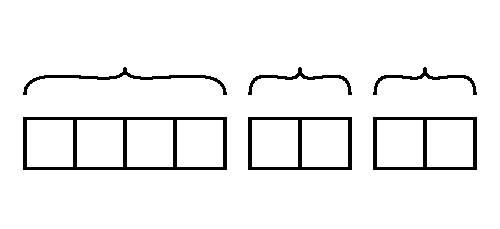
\includegraphics[scale=1]{../media/datablock.ps}\\
   % translate x=512 y=269 scale 0.38
   \putbox{0.39in}{1.12in}{1.20}{DADOS}%
   \putbox{1.72in}{1.12in}{1.20}{SEP}%
   \putbox{2.39in}{1.12in}{1.20}{CRC16}%
   \putbox{0.22in}{0.12in}{1.20}{\centbox{\midbox{0}}}%
   \putbox{0.56in}{0.12in}{1.20}{\centbox{\midbox{1}}}%
   \putbox{0.81in}{0.12in}{1.20}{}%
   \putbox{0.89in}{0.12in}{1.20}{\centbox{\midbox{2}}}%
   \putbox{1.22in}{0.12in}{1.20}{\centbox{\midbox{3}}}%
   \putbox{1.72in}{0.12in}{1.20}{\centbox{\midbox{4}}}%
   \putbox{2.06in}{0.12in}{1.20}{\centbox{\midbox{5}}}%
   \putbox{2.56in}{0.12in}{1.20}{\centbox{\midbox{6}}}%
   \putbox{2.89in}{0.12in}{1.20}{\centbox{\midbox{7}}}%
   \putbox{1.72in}{0.46in}{0.72}{\centbox{\midbox{0xFF}}}%
   \putbox{2.06in}{0.46in}{0.72}{\centbox{\midbox{0xFF}}}%
   } % close 'parbox'
   } % close 'scalebox'
   \vspace{-\baselineskip} % this is not necessary, but looks better
\end{center}

\caption{Bloco de dados para codificação}
\end{figure}

No caso de o objeto não ter o número total de bytes (4), os bytes faltantes devem ser preenchidos com zeros.
